\documentclass[tikz]{standalone}
\usetikzlibrary{shapes.geometric, decorations.markings}

\tikzset{
    mystar/.style={
        star,
        star points=6,
        inner sep=0pt,
        outer sep=0pt,
        minimum size=2cm,
        draw=black,
        fill=white
    }
}

\begin{document}
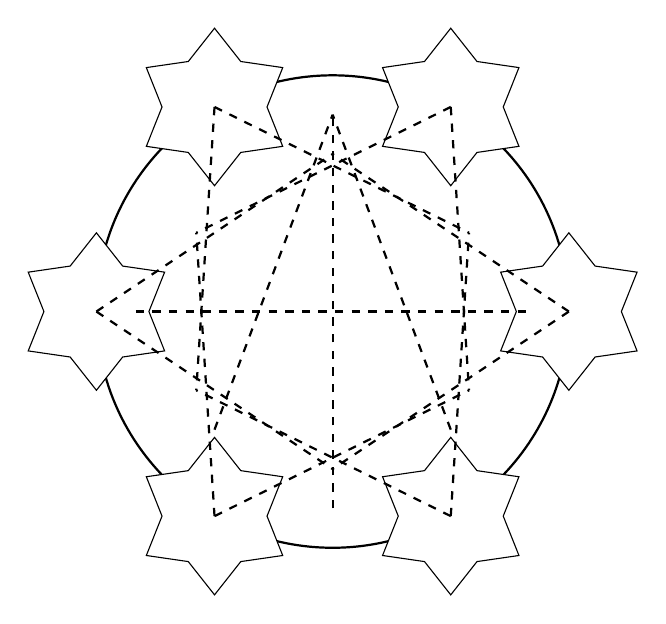
\begin{tikzpicture}[scale=1]
    % Draw the large circle at the center
    \draw[thick] (0,0) circle (3cm);

    % Draw six smaller circles surrounding the large circle
    \foreach \i in {0, 60, 120, 180, 240, 300} {
        \node[mystar] at (\i:3cm) {};
    }

    % Draw additional triangles around the large circle
    \foreach \i in {0, 60, 120, 180, 240, 300} {
        \draw[dashed, thick] (\i:3cm) -- (\i+90:2cm);
        \draw[dashed, thick] (\i:3cm) -- (\i-90:2cm);
    }

    % Draw scattered triangles throughout the design
    \draw[dashed, thick] (-1.5, -1.5) -- (0, 2.5);
    \draw[dashed, thick] (1.5, -1.5) -- (0, 2.5);
    \draw[dashed, thick] (-2.5, 0) -- (2.5, 0);
    \draw[dashed, thick] (0, -2.5) -- (0, 2.5);
\end{tikzpicture}
\end{document}